% !TEX root = main.tex
\section{Experiments}
\label{ch5-sec:experiment}


\subsection{Settings}

We use four types of data as features, including demographics, POI, geographical influence, and taxi flow, to predict the total crime rates. The details of feature data are described in Section~\ref{ch2-sec:feature}, and a description of crime data is available in Section~\ref{ch5-sec:overview}. We conduct the crime prediction on five consecutive years, 2010 -- 2014. There are over 30 categories of crime, and many categories have sparse values over regions. Therefore, we only study the effect of crime categories in Section~\ref{sec:crime-cat}, and in the rest experiments, we predict the total crime rate.

The following four methods, e.g. regression kriging (RK), linear regression (LR), negative binomial regression (NB), and geographically weighted negative binomial regression (GWNBR), are evaluated. The regression kriging method employs a regression model to incorporate all features as auxiliary variables, and then applies kriging to estimate the regression residual. We add kriging as one of the baseline, mainly because kriging is one of the most widely used method for geospatial interpolation~\cite{OlWe90}.

We evaluate the estimation accuracy under various feature combinations. The bandwidth of Gaussian kernel $h$ used for GWNBR is tuned separately under different settings. Refer to Section~\ref{sec:parameter} for more details on parameter tuning.

We adopt leave-one-out evaluation to estimate the crime rate of one geographic region given all the information of all the other regions. When we construct the spatial/social lag variable for the training data, the effect of testing region is completely removed. For example, if region $y_t$ is the testing region, the remaining $\{y_i | \forall i \text{ s.t. } i \neq t\}$ become the training set. For any $y_i$ in the training set, its geographical influence feature and taxi flow feature are constructed only from $\{y_i | \forall i \text{ s.t. } i \neq t\}$.

In the evaluation, we estimate the crime rate for testing community areas. The accuracy of estimation is evaluated by mean absolute error (MAE) and mean relative error (MRE).

\begin{align}
MAE & = \frac{\sum_i |y_i - \hat{y_i}| }{n} \\
MRE & = \frac{\sum_i |y_i - \hat{y_i}|} {\sum_i y_i }
\end{align}



\begin{table}
\centering
\caption{Performance evaluation on total crime rate prediction. Various feature combinations are shown in each column. The linear regression model,  negative binomial model, and geographically weighted negative binomial model are compared by year group. }
\label{tb:perf}

\resizebox{!}{0.45\textheight}{
\begin{tabular}{|c|c|c|c|c|c|c|}
\hline
\multicolumn{3}{|c|}{} & \multicolumn{4}{|c|}{Settings} \\ \hline
\multicolumn{3}{|c|}{Column ID} & 1 & 2 & 3 & 4  \\ \hline
\multicolumn{2}{|c|}{\multirow{4}{*}{Features$^1$}}	& \textbf{D}emo &  \checkmark& \checkmark& \checkmark& \checkmark \\ \cline{3-7}
\multicolumn{2}{|c|}{}	& \textbf{G}eo & \checkmark & \checkmark& \checkmark& \checkmark \\ \cline{3-7}
\multicolumn{2}{|c|}{}	& \textbf{P}OI & &\checkmark & & \checkmark \\ \cline{3-7}
\multicolumn{2}{|c|}{}	& \textbf{T}axi & & & \checkmark& \checkmark \\ \hline
Year & Model$^2$ & Error & \multicolumn{4}{|c|}{} \\ \hline
                       &  & MAE & 463.68 & 461.67 & 452.39 & 421.59 \\ \cline{3-7}
                       & \multirow{-2}{*}{RK} & MRE & 0.346 & 0.344 & 0.337 & 0.314 \\ \hhline{|~|*{6}{-|}}
  \rowcolor{Gray}  
  \cellcolor{white} &  \cellcolor{white} & MAE &  394.78 & 432.45 & 413.80 & 404.00\\ \hhline{|~|~|*{5}{-|}}
  \rowcolor{Gray}
  \cellcolor{white} & \cellcolor{white}\multirow{-2}{*}{LR}& MRE &  0.295 & 0.323 & 0.309 & 0.301\\ \hhline{|~|*{6}{-|}}
	
                       &  & MAE &  402.82 & 343.55 & 404.49  & 315.28\\ \cline{3-7}
                       & \multirow{-2}{*}{NB}	& MRE  & 0.301 & 0.256 & 0.302 & 0.235 \\ \hhline{|~|*{6}{-|}}
  \rowcolor{Gray2}
  \cellcolor{white}	& \cellcolor{white} & MAE & 343.44 & 332.38 & 327.20 & \textbf{265.93}\\ \hhline{|~|~|*{5}{-|}}
  \rowcolor{Gray2}
  \cellcolor{white}\multirow{-8}{*}{2010} & \cellcolor{white}\multirow{-2}{*}{GWNBR} & MRE & 0.256 & 0.248 & 0.244 & \textbf{0.198} \\ \hline
	
                       &  & MAE & 460.83 & 422.01 & 424.05 & 430.77 \\ \cline{3-7}
                       & \multirow{-2}{*}{RK} & MRE & 0.358 & 0.328 & 0.330 & 0.335 \\ \hhline{|~|*{6}{-|}}
  \rowcolor{Gray}  
  \cellcolor{white} & \cellcolor{white} & MAE & 380.08 & 422.94 & 402.63 & 402.81\\  \hhline{|~|~|*{5}{-|}}
  \rowcolor{Gray}
  \cellcolor{white} & \cellcolor{white}\multirow{-2}{*}{LR}& MRE & 0.296 & 0.329 & 0.313 & 0.313\\ \hhline{|~|*{6}{-|}}
                       & & MAE & 391.26 & 340.49  & 396.59  & 325.34 \\ \cline{3-7}
                       & \multirow{-2}{*}{NB}	& MRE  & 0.304 & 0.265  & 0.308  & 0.253 \\ \hhline{|~|*{6}{-|}}
  \rowcolor{Gray2}
  \cellcolor{white}	& \cellcolor{white} & MAE & 330.04 & 325.56 & 322.77  & \textbf{275.61}\\ \hhline{|~|~|*{5}{-|}}
  \rowcolor{Gray2}
  \cellcolor{white}\multirow{-8}{*}{2011}	&\cellcolor{white}\multirow{-2}{*}{GWNBR}	& MRE  & 0.257 & 0.253 & 0.251 & \textbf{0.214} \\ \hline

                       & & MAE & 455.94 & 418.04 & 438.13 & 412.55 \\ \cline{3-7}
                       & \multirow{-2}{*}{RK} & MRE & 0.368 & 0.338 & 0.354 & 0.333 \\ \hhline{|~|*{6}{-|}}
  \rowcolor{Gray}
  \cellcolor{white} &  \cellcolor{white} & MAE & 375.62 & 423.88 & 402.69 & 404.06\\ \hhline{|~|~|*{5}{-|}}
  \rowcolor{Gray}
  \cellcolor{white} & \cellcolor{white}\multirow{-2}{*}{LR}& MRE & 0.304 & 0.343 & 0.325 & 0.327\\ \hhline{|~|*{6}{-|}}

                       & & MAE & 395.82 & 349.09 & 399.99 & 342.41  \\ \cline{3-7}
                       & \multirow{-2}{*}{NB}	& MRE  & 0.320 & 0.282  & 0.323  & 0.277  \\ \hhline{|~|*{6}{-|}}
		\rowcolor{Gray2}
		\cellcolor{white}	& \cellcolor{white} & MAE  & 332.70 & 342.95 & 334.83 & \textbf{330.51} \\ \hhline{|~|~|*{5}{-|}}
		\rowcolor{Gray2}
		\cellcolor{white}\multirow{-8}{*}{2012}	&\cellcolor{white}\multirow{-2}{*}{GWNBR}	& MRE  &0.269  & 0.277 & 0.270 & \textbf{0.267} \\ \hline
	
                       & & MAE & 408.90 & 468.39 & 457.20 & 413.77 \\ \cline{3-7}
                       & \multirow{-2}{*}{RK} & MRE & 0.360 & 0.412 & 0.402 & 0.363 \\ \hhline{|~|*{6}{-|}}
  \rowcolor{Gray}
  \cellcolor{white} & \cellcolor{white} & MAE & 369.24 & 433.48 & 387.58 & 400.75\\ \hhline{|~|~|*{5}{-|}}
  \rowcolor{Gray}
  \cellcolor{white} & \cellcolor{white}\multirow{-2}{*}{LR}& MRE & 0.325 & 0.381 & 0.341 & 0.352\\ \hhline{|~|*{6}{-|}}
                       &  & MAE & 390.09 & 348.16 & 389.79 & 324.94 \\ \cline{3-7}
                       & \multirow{-2}{*}{NB}	& MRE & 0.343 & 0.306  & 0.343  & 0.286 \\ \hhline{|~|*{6}{-|}}
  \rowcolor{Gray2}
  \cellcolor{white}	& \cellcolor{white} & MAE & 319.75 & 334.58  & 316.70 & \textbf{316.34}\\ \hhline{|~|~|*{5}{-|}}
  \rowcolor{Gray2}
  \cellcolor{white}\multirow{-8}{*}{2013}	&\cellcolor{white}\multirow{-2}{*}{GWNBR}	& MRE   & 0.281 & 0.294 & 0.279 & \textbf{0.278} \\ \hline
	
                       & & MAE & 404.76 & 365.14 & 453.07 & 380.83 \\ \cline{3-7}
                       & \multirow{-2}{*}{RK} & MRE & 0.398 & 0.359 & 0.446 & 0.374 \\ \hhline{|~|*{6}{-|}}
  \rowcolor{Gray}
  \cellcolor{white} & \cellcolor{white} & MAE & 329.93 & 386.9 & 355.83 & 358.47\\ \hhline{|~|~|*{5}{-|}}
  \rowcolor{Gray}
  \cellcolor{white} & \cellcolor{white}\multirow{-2}{*}{LR}& MRE &   0.325 & 0.381 & 0.35 & 0.353\\ \hhline{|~|*{6}{-|}}

                       &  & MAE & 347.39 & 303.59  & 348.71  & 289.52\\ \cline{3-7}
                       & \multirow{-2}{*}{NB} & MRE & 0.342  & 0.299  & 0.343  & 0.285 \\ \hhline{|~|*{6}{-|}}
  \rowcolor{Gray2}
  \cellcolor{white}	& \cellcolor{white} & MAE & 282.35  & 280.58  & 274.16  & \textbf{272.51}\\ \hhline{|~|~|*{5}{-|}}
  \rowcolor{Gray2}
  \cellcolor{white}\multirow{-8}{*}{2014}	&\cellcolor{white}\multirow{-2}{*}{GWNBR} & MRE & 0.277  & 0.276 & 0.270 & \textbf{0.268} \\ \hline
\end{tabular}
}

\footnotesize{$^1$ Demo -- demographic features, Geo -- geographical influence, POI -- POI features, Taxi -- taxi flow feature.}
\footnotesize{$^2$ RK -- Regression Kriging, LR -- Linear Regression, NB -- Negative Binomial Regression, GWNBR -- Geographically Weighted Negative Binomial Regression.}
\end{table}



\subsection{Performance on Different Feature Combinations}

The leave-one-out evaluation results are shown in Table~\ref{tb:perf}. Ideally, we should show all the possible combinations of feature groups, which will result in 15 combinations. Due to the space limit, we show 4 combinations in Table~\ref{tb:perf}. Setting 1 (\textbf{D+G}) represents the traditional features used in criminology literature. Setting 2 (\textbf{D+G+P}) and setting 3 (\textbf{D+G+T}) are used to examine the individual effects of new features on POI and Taxi flows. Setting 4 (\textbf{D+G+P+T}) studies the combined effects of all features.

\subsubsection{POI Feature} 
Adding POI features improves the accuracy of the NB model (see setting 2 vs. setting 1 and setting 4 vs. setting 3 in Table~\ref{tb:perf}). The POI distribution reflects the functionality of a region. The most correlated POI major category is ``professional'', under which there are a lot of venues like transportation center and conventional center. These are locations with more dynamic movements of people. Such location information is not reflected in any of other features. POI thus provides  unique information and it shows that using big data can benefit us in advancing the study of traditional crime inference problems. 

Another issue worth discussing is whether POI is a surrogate of population features from demographics. That is, a region with more POIs is a region with higher population. However, as we see from Table~\ref{tb:perf}, the NB model using POI feature in addition to the demographic and geographic features always outperforms the model without the POI feature. This is because population from demographics reflects the number of residents in that region, but POI reflects dynamics of population (e.g., people go to venues for food, entertainment, or travel). Therefore, the dynamic population in POI further complements the residential population in demographics.


\subsubsection{Taxi Flow} 
%The taxi flow is shown to improve the inference accuracy (see Table~\ref{tb:perf} for column 3 vs. column 1 and column 4 vs. column 2). This validates our hypothesis that crimes do not only correlate with nearby regions but also correlate through hyperlinks on the space (i.e., the taxi flow). 

To test our hypothesis that crimes do not only correlate with nearby regions but also correlate through hyperlinks on the space (i.e., the taxi flow), we examine if considering taxi flow improves the inference accuracy. Comparing setting 3 with setting 1 in Table~\ref{tb:perf}, we find that the improvement by taxi flow is not obvious for NB. However, comparing setting 4 with setting 2, we observe a much more significant accuracy boost. The reason could be that the taxi flow further complements the POI data. When POI information is missing from the predictor, the city dynamics captured by taxi flow are weakened as well.

Meanwhile, we note that incorporating the new urban data (POIs and taxi flow) significantly improves the performance of the NB model. Specifically, comparing  setting 4 with setting 1, the improvements in MRE are 6.6\%, 5.1\%, 4.3\%, 5.7\%, and 5.7\% for the five years, respectively.


\subsubsection{Feature Consistency}

In this section, we study the consistency of features as shown in Figure~\ref{fig:fcon}. We get the effect of adding POI feature by comparing setting 2 and setting 1 in Table~\ref{tb:perf}. Similarly, setting 3 vs setting 1 shows the effect of adding taxi, and setting 4 vs setting 1 shows the effect of adding both. For each method we show number of years in y-axis, in which the added feature improves the model performance.

We observe that adding both features shows the best performance for both NB and GWNBR, meanwhile it is not necessarily the best for other models. For example, LR shows that setting 1 is better than setting 4 over different years. RK shows that setting 1 is better than setting 4 in year 2013 but not other years. We argue that it is crucial to use the right model to captures extra information and achieves consistent results.

\begin{figure}[t]
\centering
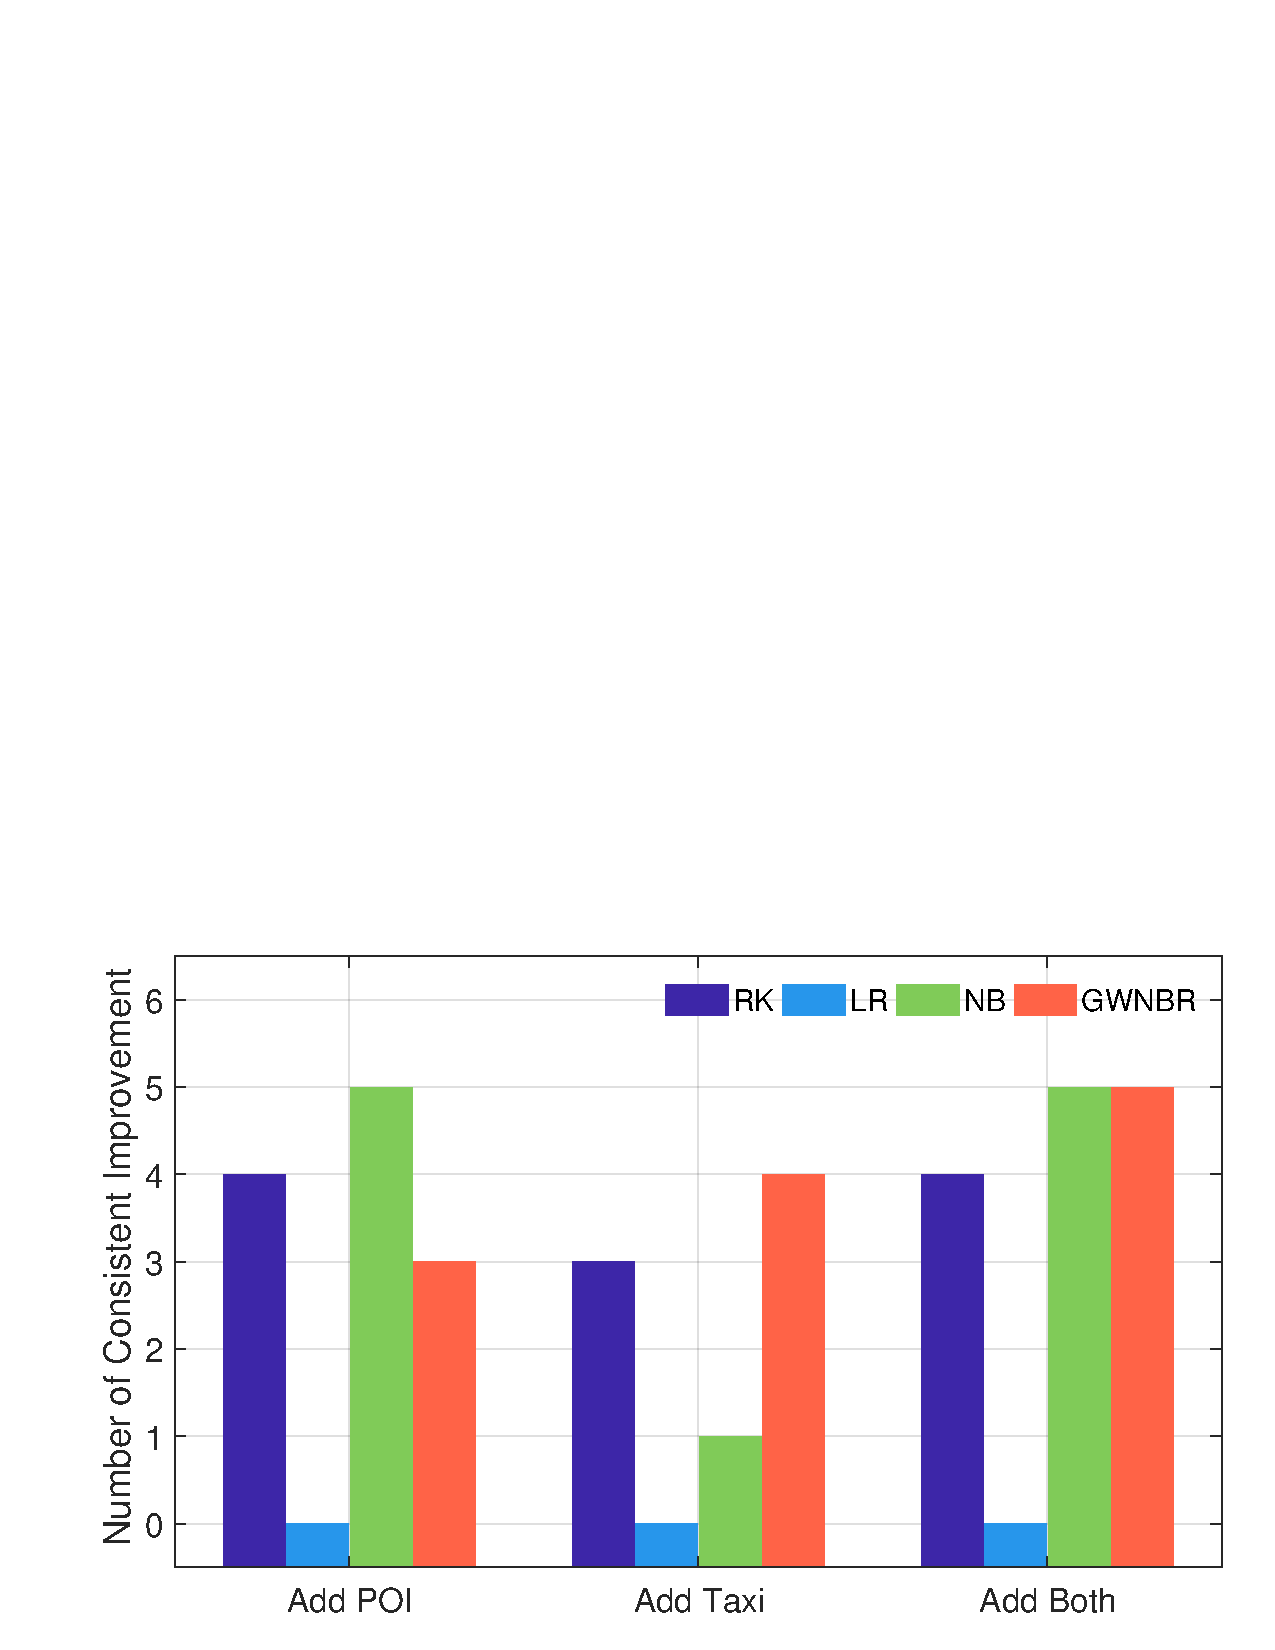
\includegraphics[width=0.7\linewidth]{fig/feature_consistency.pdf}
\caption{The feature consistency results. The x-axis shows the effect of adding different features. The y-axis shows number of years that shows improvement.}
\label{fig:fcon}
\vspace{-3mm}
\end{figure}




\subsection{Performance on Different Methods}

In this section, we compare the prediction error of different methods, and we have the following observations.

\subsubsection{Regression Kriging vs. Other Regressions}
We observe that kriging method usually performs worse than other regression methods. The reason is that the kriging method is designed for interpolation and the objective is to minimize the estimation variance. Kriging method usually overestimates a local minimum and underestimates a local maximum due to the fact the kriging uses average to interpolate. For the crime rate prediction problem, other regression methods directly optimize the prediction error, and therefore outperforms the kriging method.

\subsubsection{Negative Binomial Regression vs. Linear Regression}
In Table~\ref{tb:perf},  we can see that under most settings, the negative binomial regression significantly outperforms the linear regression (with only a few exceptions when using demographic features and geographic features). When using all the features, NB is significantly better than LR with at least $5\%$ improvement in MRE.
There are two reasons why the negative binomial regression is more appropriate for crime rate estimation than linear regression.
First, negative binomial regression guarantees the prediction variable is non-negative. Second, it is difficult to get very precise estimates of crime rate, and the negative binomial regression allows a large variance in the estimated crime rate. 


\subsubsection{GWNBR vs. NB, and the Effectiveness of Non-Stationary Model}
Next, we compare the negative binomial regression with the geographically weighed negative binomial regression. As shown in~Table~\ref{tb:perf}, the GWNBR model consistently outperforms the NB model in all experiment settings, which validate our hypothesis that the correlation among crime rate and other features are non-stationary. 

In addition, comparing setting 2 (\textbf{D+G+P}) or setting 3 (\textbf{D+G+T}) with setting 1 (\textbf{D+G}) in Table~\ref{tb:perf}, we observe that the performance improvement for GWNBR by POI feature or taxi flow separately is not obvious. However, when all features (\textbf{D+G+P+T}) are used, GWNBR consistently gives lower estimation error than using the traditional features only (\textbf{D+G}). In the best case (years 2010 and 2011), GWNBR reduces the MAE by over 15\%. This again suggests that the POI feature and taxi flow complement each other, and that incorporating both features yields the best inference accuracy.


In view of the superior performance of GWNBR, in all the following experiments we only refer to the performance of GWNBR.


\subsection{Parameter Sensitivity}
\label{sec:parameter}

In the GWNBR model, the bandwidth parameter $h$ in Equation~(\ref{eq:gwr-gkn}) controls the influence of a nearby training sample. There are several approaches to determine the bandwidth $h$~\cite{WLL+15}. Here, we adopt the cross validation approach to estimate a best $h$ from data. More specifically, we fit a model on the training data and report the prediction error on the testing data. The best $h$ should lead to the lowest prediction error.


In this experiment, we use data from year 2010 to study the effect the bandwidth $h$ on the performance of GWNBR. Using a data-driven approach, we adopt the mean absolute error as a measure of fit. In Figure~\ref{fig:gwnbr-h}, we plot the MAE against bandwidth under leave-one-out setting. It is clear that the optimal bandwidth is $5.8$, which gives us the lowest MAE. Furthermore, we observe that when $h$ becomes larger, the performance of GWNBR model approaches to the NB model (with a MAE of $310$). This observation is consistent with the model, because an infinitely large bandwidth gives all samples the same weight, which makes the GWNBR essentially  an NB model. 

\begin{figure}[h]
	\centering
	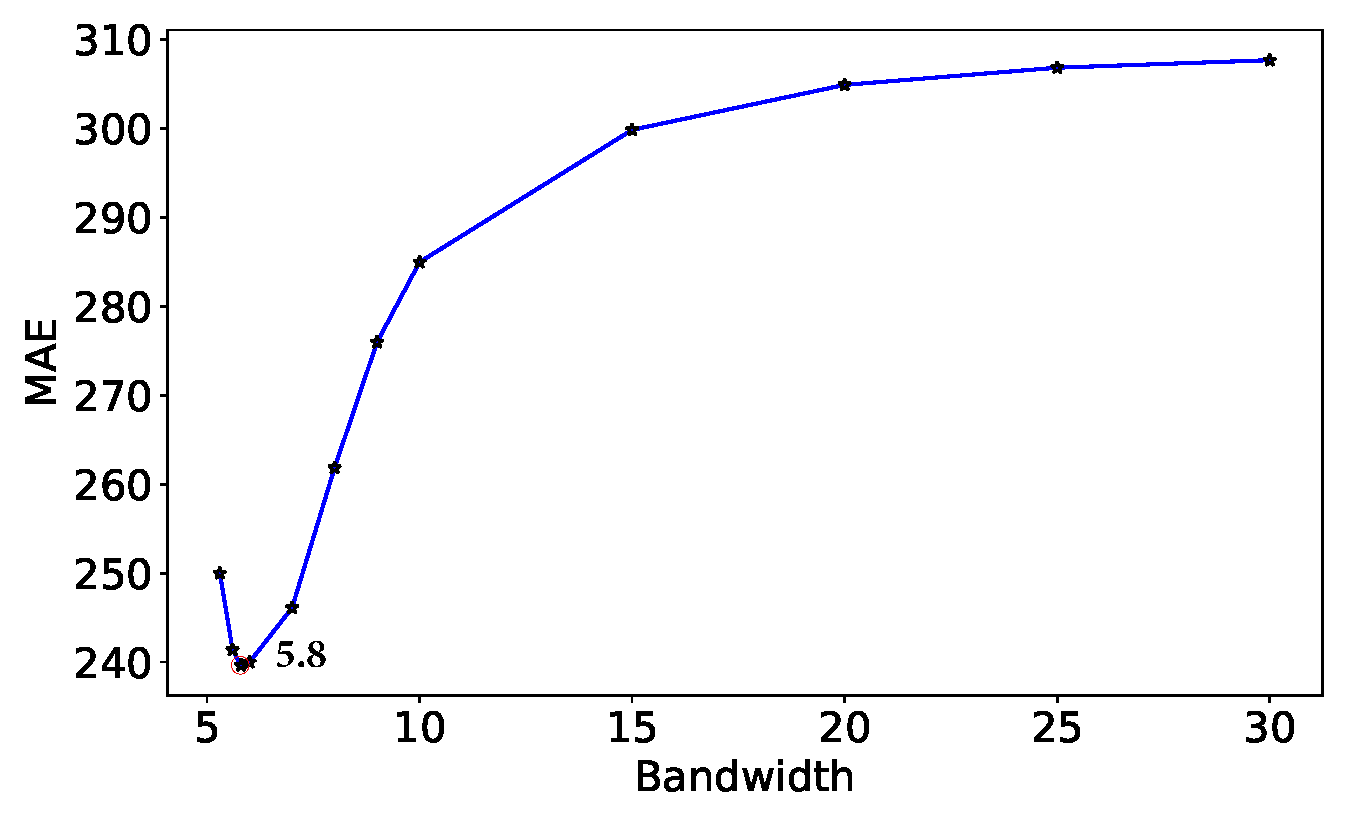
\includegraphics[width=0.7\linewidth]{fig/para_sensitive.pdf}
	\caption{Bandwidth sensitivity analysis for geographically weighted negative binomial regression.}
	\label{fig:gwnbr-h}
\vspace{-3mm}
\end{figure}




%\medskip
%\noindent \textbf{Taxi Flow normalization.} 
\nop{
\subsubsection{Taxi Flow Normalization}
The taxi flow represents the interactions among community areas. There are several different approaches to incorporate the taxi flow into the model.  First, we can use the raw taxi count as a weight on crime from other neighborhoods. One issue with the raw count is the concentration of taxi trips distribution in the downtown area. Consider the following example. In the downtown area, the average taxi flow count is \num{1000} between any pair of community areas, while the average of suburbs is $100$. When we propagate crime by raw taxi count, the same amount of crime in downtown is propagated with a  $10$ times higher coefficient than that of suburb. 


To address this issue, we can normalize the taxi flow, and there are two different approaches to normalize. 1) We can normalize the taxi flow by the total incoming traffic of the destination community area, and the semantics of this normalization is splitting the crime in the destination to all its neighbors. 2) Alternatively, we can normalize the taxi flow by the outgoing total trips in the source community area. This normalization assumes the crime in each source community is spread out by the flow.  The two normalization methods are shown in Figure~\ref{fig:taxiflow-norm}.


\begin{figure}[h]
\centering
\begin{tikzpicture}
\node[right]  at (0,0) {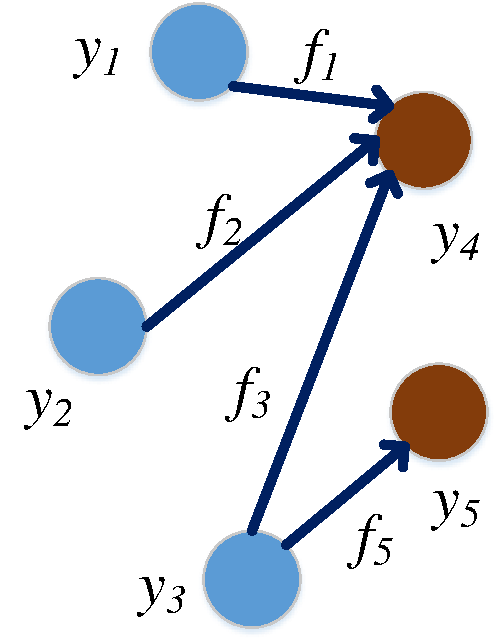
\includegraphics[width=0.12\textwidth]{fig/taxiflow-normalization.pdf}};
\node[align=left, above right] at (2.3, 0.3) {Normalization by source: \\ $F^t_4 = \frac{f_1}{f_1} y_1 + \frac{f_2}{f_2} y_2 + \frac{f_3}{f_3+f_5} y_3$};
\node[align=left, below right] at (2.3, -0.3) {Normalization by destination:  \\ $F^t_4 = \frac{f_1}{f_1+f_2+f_3} y_1 + \frac{f_2}{f_1+f_2+f_3} y_2 + \frac{f_3}{f_1+f_2+f_3} y_3$};
\end{tikzpicture}
\caption{Two different normalization schemes.}
\label{fig:taxiflow-norm}
\end{figure}



\begin{table}[h]
\centering
\caption{Various approaches to construct taxi flow feature. Estimation for crime in 2013 with all other features.}{
\label{tb:tf-design}
\begin{tabular}{|l|c|c|}
\hline
\multirow{2}{*}{Settings} & \multicolumn{2}{|c|}{GWNBR} \\ \cline{2-3}
	& MAE & MRE \\ \hline
Taxi flow count & 364.02 & 0.320 \\ \hline
Taxi flow normalized by source & 324.15 & 0.285 \\ \hline
Taxi flow normalized by destination & 304.26& 0.268\\ \hline
\end{tabular}}
\end{table}


In Table~\ref{tb:tf-design} we compare the different approaches to handle the taxi flow. Using raw taxi flow count is clearly not a good option, due to the unbalanced data distribution. We also observe that normalizing taxi flow by destination is better than normalization by source. The reason could be explained by the example given in Figure~\ref{fig:taxiflow-norm}. Suppose the focal region is a transportation hub, which has a lot of isolated regions connected to it. If we normalize the crime by source region, then the taxi flow feature of focal region is overestimated, since the coefficients of its neighbors do not sum to one. 
}



\subsection{Feature Importance}

In this section, we study the importance of features through significance tests.


From previous results, we see that combining POI features and taxi flow will help improve the estimation accuracy. Now we try to measure the significance of this accuracy boost by permutation tests. If a feature correlates with crime, when we randomly permute the values of this feature among neighborhoods, we will expect a higher error in crime rate estimation. So in each round of permutation, we can get an error in estimation. We compare the error with the original feature to the error distribution obtained from permutations. We conduct 1,000 rounds of permutations to approximately estimate the error distribution. The position of the original error in this distribution indicates the significance of this feature. For example, if the original error is smaller than 99\% of the errors from the permutations, the p-value is 0.01. 

\nop{
The permutation test procedure is described as follows. Each feature is randomly permuted for $1,000$ times. After each permutation, the leave one out evaluation is applied to get the accuracy measure (MAE, MRE). The $1,000$ rounds leave-one-out give us the distribution of accuracy measure under the null hypothesis that the permuted feature is irrelevant to the crime. We further calculate the probability that under the null hypothesis the error is smaller than the error in Table~\ref{tb:perf}, and this probability is our p-value.  }


\begin{table}
\centering
\caption{Estimated p-value for each feature. The p-value is defined as the possibility that a smaller error measure is observed under the null hypothesis. Permutation test is conducted on 2014 data with all features (D+G+P+T) used.}
\label{tb:permt}
\begin{tabular}{|c|c|c|c|c|c|c|}
\hline
\multirow{3}{*}{\makecell{Settings: \\D+G+P+T}} & \multicolumn{2}{c}{LR} & \multicolumn{2}{|c|}{NB} & \multicolumn{2}{|c|}{GWNBR}\\ \cline{2-7}
	& MAE & MRE & MAE & MRE & MAE & MRE \\ \cline{2-7}
	& 358.47 & 0.353 & 289.52 & 0.285 & 272.51 & 0.268\\ \hline
Feature & \multicolumn{6}{c|}{p-value} \\ \hline
D & 0.000 & 0.000 & 0.000 & 0.000 & 0.000 & 0.000\\ \hline 
G & 0.001 & 0.001 & 0.005 & 0.005 & 0.004 & 0.004  \\ \hline
P & 0.022 & 0.021 & 0.005 & 0.005 & 0.006 & 0.007\\ \hline
T & 0.000 & 0.000 & 0.080 & 0.079 & 0.049 & 0.052\\ \hline
\end{tabular}
\vspace{-3mm}
\end{table}


In Table~\ref{tb:permt}, the p-values of different features are reported. The demographics feature is the most significant feature with estimated p-value being $0.00$. In all the $1,000$ random permutations of demographic feature, we never observe an error lower than the original error.  The proposed POI distribution and taxi flow are significant as well, with  p-values of $0.6\%$ and $4.9\%$ for the GWNBR.  We notice that the taxi flow has a p-value around $5\%$ instead of close to $0$. One reason is that the taxi flow overlaps with geographic feature. Thus, permuting taxi flow may not have a critical influence on the estimation error in certain cases.

%\footnotetext{The taxi flow feature significance is not exactly the same as KDD paper, because we updated the taxi flow within a different time period. The observations on taxi flow are consistent with KDD. The geographic feature differs a lot from KDD paper. In KDD paper, we report geographic feature  not significant (with a p-value of $0.6$. This is due to an error in KDD submission. Here we correct this error, and geographic feature is significant with a p-value of $0.005$.}


\nop{
\subsubsection{Coefficient Study}

In our regression model, the coefficient also indicates the importance of features. We normalize the values of all features to the range $[0,1]$, so that coefficients are comparable. Note that, under the GWNBR setting, there are multiple models in one year. Therefore, we further compute the average coefficient of all the models within the same year. This average coefficient is meaningful, because all the models are trained on the same data samples with different weights. In Eq.~(\ref{eq:gwr-general}), the weight $\gamma_{ij}$ is applied on the error term, thus does not change the importance of any specific feature.  The top-6 features with the most significant coefficients are shown in Table~\ref{tb:fea-stability}. The top three rows in Table~\ref{tb:fea-stability} are features with positive coefficients, which implies positive correlations with the crime rate. The bottom three features are negatively correlated with the crime rate.

By comparing the coefficients over different years, we observe that the coefficients are relatively stable with respect to time. The most important feature is percentage black, which captures the demographics of residents. The other two important features are POI outdoors and POI food. We also find three POI categories are among the top negatively correlated features. They are shop, residence, and education categories. The reason is probably that 1) at those places the population is relatively stable such as residence, which provides less opportunity for crime; 2) those places have taken precautions against crime, such as shop.
 

\begin{table}[h]
\centering
\caption{The coefficients of the top-6 features over different years. There are 21 different features in total. We only show the top-3 features with the highest positive/negative coefficients, respectively.}
\label{tb:fea-stability}
\scalebox{0.9}{
	\begin{tabular}{|c|c|c|c|c|c|}
	\hline
	\multirow{2}{*}{Feature} & \multicolumn{5}{c|}{Year} \\ \cline{2-6}
		& 2010 & 2011 & 2012 & 2013 & 2014 \\ \hline \hline
	Percentage black & 0.662 & 0.698 & 0.762 & 0.724 & 0.532             \\ \hline
	POI outdoors recreation & 0.617 & 0.641 & 0.607 & 0.564 &0.850       \\ \hline
	POI food & 0.423 & 0.531 & 0.547 & 0.499 & 0.484   \\ \hline \hline
	POI education &-0.269 &-0.307 &-0.369 &-0.393 &-0.360   \\ \hline
	POI residence & -0.188 &-0.328 &-0.364 &-0.285 &-0.366   \\ \hline
	POI shops &-0.397 &-0.478 &-0.520 &-0.446 &-0.515        \\ \hline
	\end{tabular}
}
\end{table}
}


\subsection{Improvements in Different Regions}

The POI distributions and taxi flow patterns are different from region to region. It is interesting to find out whether they have a consistently positive impact in crime rate estimation. For POI feature, we calculate the difference in estimation error (MAE) between two setting 3 (D+G+T) and setting 4 (D+G+P+T). Similarly, the MAE difference between setting 2 and setting 4 is calculated for the taxi flow feature. The results are shown in Figure~\ref{fig:feat-area}.  A positive difference (blue area) indicates that adding the new feature helps reduce the estimation error, while a negative difference (red area) indicates that the new feature adds more noise to the data.  

\begin{figure}[h!]
\centering
\subfigure[POI]{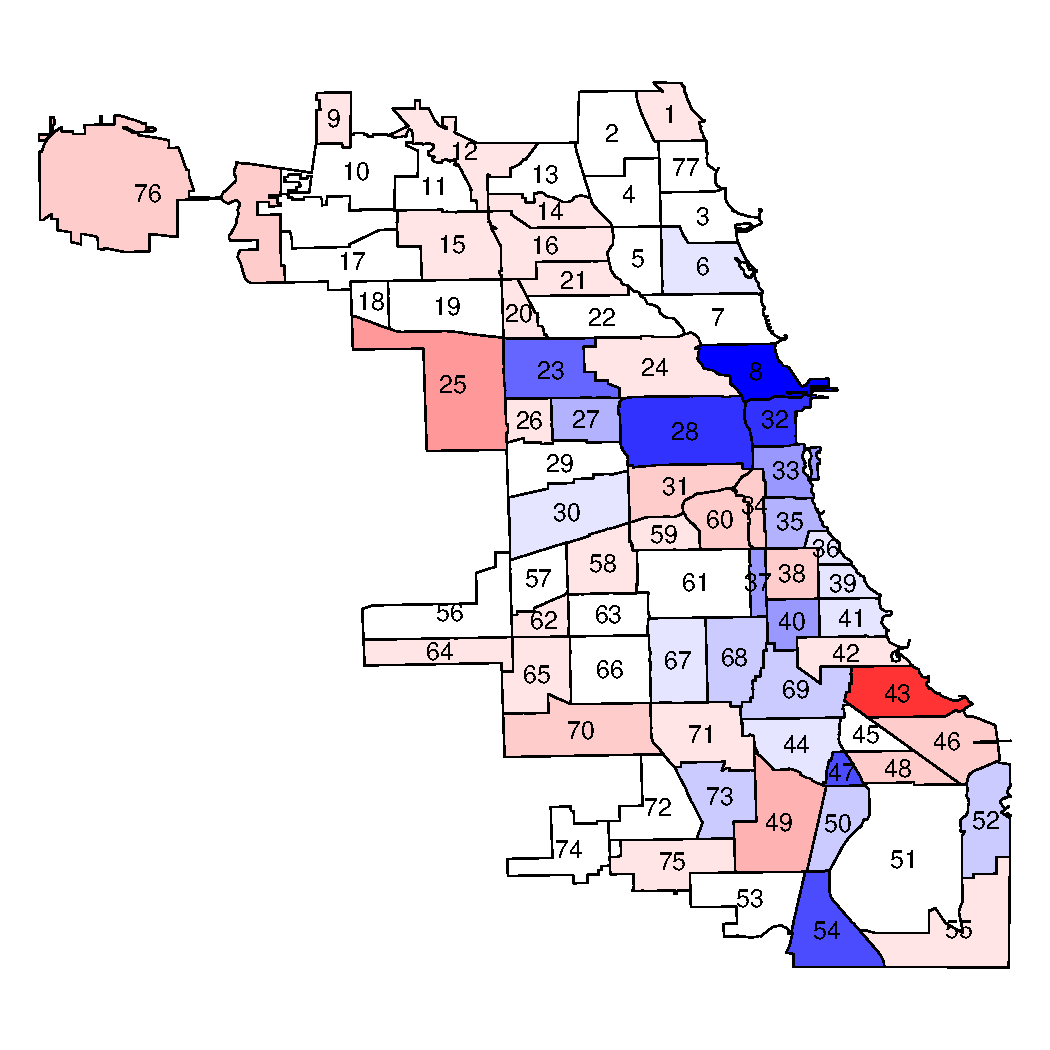
\includegraphics[width=0.45\linewidth]{fig/poi-improve_2014_new.pdf}}
\subfigure[Taxi flow]{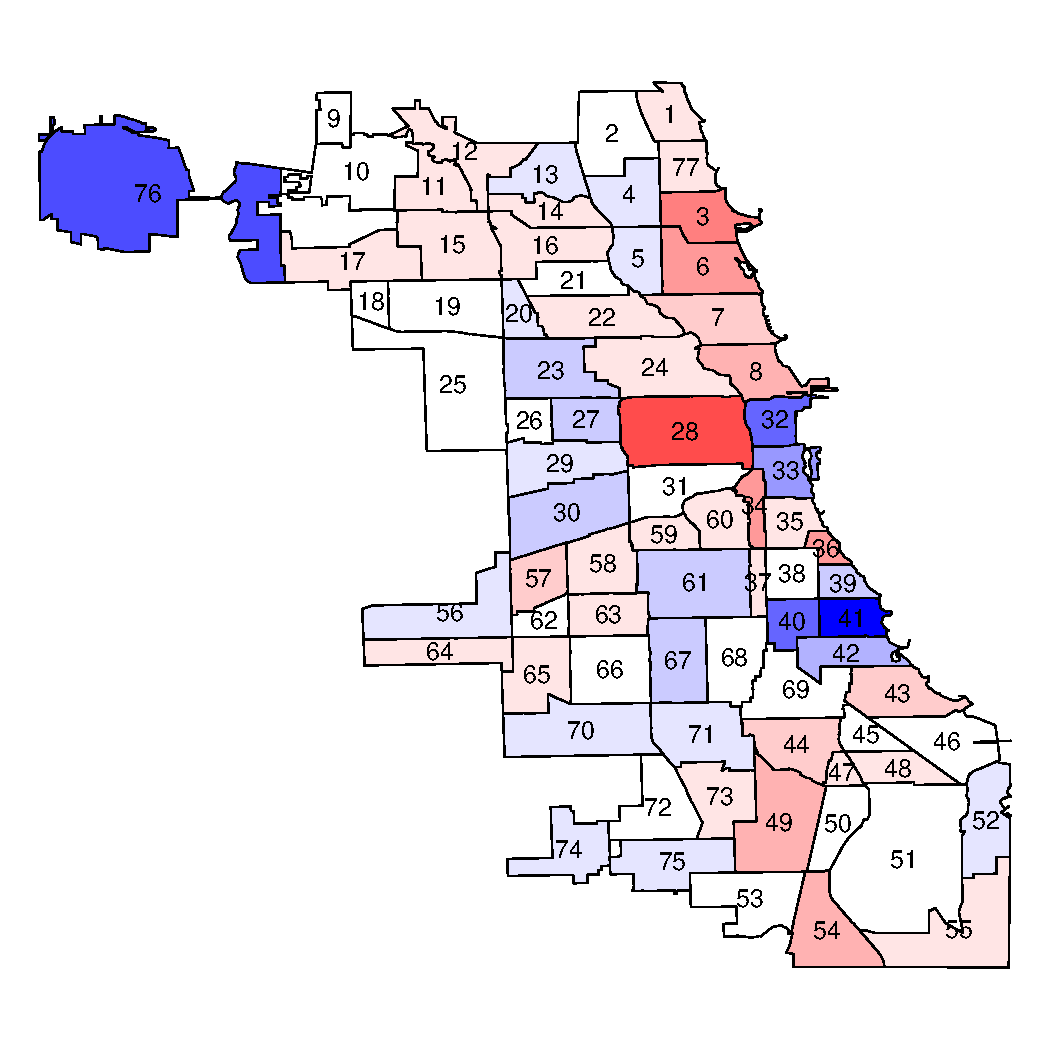
\includegraphics[width=0.45\linewidth]{fig/taxi-improve_2014_new.pdf}}
\caption{Performance improvement per region in year 2014. \textbf{Left:} The MAE difference of setting 3 and 4. \textbf{Right} The MAE difference of setting 2 and 4. The color blue means the MAE is reduced by adding the corresponding feature, while color red means the MAE is increased. The color saturation indicates the value of difference.}
\label{fig:feat-area}
\end{figure}


It is interesting to observe that in the downtown area, i.e. community areas \#8, \#32, and \#28, POI significantly improves the estimation accuracy. The reason is two fold. 1) The demographics information from census is mostly about the residing population in the focal area.  However, in the downtown area there are a lot of floating population groups conducting various social activities, and this is not reflected by the census demographics. The POI information, on the other hand, reflects the functionality of a region, hence complements the demographic information. 2) In the downtown area, there are more POIs than other places, which provide more complete information about the community profile.

As for the taxi flow feature, it helps the most in those suburb area, because the taxi flow reflects the social interaction in those areas. In the downtown area \#28 and \#8, the taxi flow feature incurs a relatively large estimation error. The reason is that the taxi flow distribution in Chicago is extremely skewed. Roughly 61\% of the Chicago taxi trips have a destination in the downtown area, which may result in the model over-propagating crime estimates from all of Chicago into the downtown area.



